\documentclass[long, final]{jobim}
% Available options are:
% - showframe
% - draft
% - final [default]

\usepackage[utf8]{inputenc}

% WARNING: already loaded packages:
% - hyperref
% - times
% - color
% - xspace
% - graphicx
% - fancyhdr
% - fancybox
% - indentfirst
% - geometry
% - babel (options english,francais) :
%   choose the language with \selectlanguage{<language>}
\usepackage{svg}
\usepackage{pifont}
\usepackage{xcolor}
\usepackage{tcolorbox}
\usepackage{tikz}
\usepackage{pgfplots}
\usepackage{wrapfig}
\usepackage{multicol}
\usepackage{ragged2e}
\usepackage{amsmath}
\usepackage{amsfonts}

\usetikzlibrary{calc,fit,shapes.arrows,positioning}
\usetikzlibrary{graphs}
\usetikzlibrary{graphdrawing}
\usetikzlibrary{trees,matrix}
\usegdlibrary{trees}

\colorlet{darkyellow}{yellow!60!black}
\colorlet{lightblue}{blue!65}
\colorlet{darkred}{red!60!black}

\definecolor{mycolor}{rgb}{0.122, 0.435, 0.698}
\definecolor{mycolor}{rgb}{0.122, 0.435, 0.698}
\newtcbox{\mybox}{on line,
  colframe=mycolor,colback=mycolor!10!white,arc=4pt,boxsep=0pt,left=3pt,right=3pt,boxrule=0pt,top=3pt,bottom=3pt}
\newcommand{\realemph}[1]{\mybox{\textit{#1}}}

\pagestyle{empty}
\addtolength{\parskip}{0.4\baselineskip}

%% Title of the paper (required)
\title{Bringing ABC inference to the machine learning realm : AbcRanger, an optimized random forests library for ABC}

%% List of authors (separated by the macro \and).
%% Authors can be followed by \inst{<n>} macro.
%% The <n> parameter of the \inst macro should correspond to the <n>th institution
%% (see macro \institute below).
\author{François-David \textsc{Collin}\inst{1} \and Arnaud \textsc{Estoup}\inst{2} \and Jean-Michel \textsc{Marin}\inst{1} \and Louis \textsc{Raynal}\inst{1}}

%% List of institutions (separated by the macro \and).
\institute{
  Université de Montpellier, CNRS, IMAG UMR 5149, Montpellier, France
 \and
 CBGP, INRA, CIRAD, IRD, Montpellier SupAgro, Univ. Montpellier, Montpellier, France
}

% email of the corresponding author
\corresponding{Francois-David.Collin@umontpellier.fr@umontpellier.fr}

% Enter the reference of your paper
\papername{Meert \textit{et al.} (2016) Unknown species discovered by metagenomics
  of frikandels. \textit{Annals of Improbable Research}. \url{http://dx.doi.org/11.0110/0111/111-1110-0001}}

%% Abstract of the paper (required).
\abstract{%
The \href{https://github.com/diyabc/abcranger}{AbcRanger library} provides methodologies for model choice and parameter estimation based on fast and scalable \emph{Random Forests}, tuned to handle large and/or high dimensional datasets. The library, initially intended for the population genetics ABC framework \href{https://github.com/diyabc/diyabc}{DIYABC}, has been generalized to any ABC reference table generator.

At first, computational issues were encountered with the reference ABC-Random Forest. Those issues have been diagnosed by us as friction between "strict" Machine Learning setup and ABC context, and this incited us to modify the C++ implementation of state-of-the-art random forests, \href{https://github.com/imbs-hl/ranger}{ranger}, to tailor it for ABC needs: potentially "deep" decision trees are not stored in memory anymore, but are processed by batches in parallel.

We focused on memory and thread scalability, ease of use (minimal hyperparameter set).
R and python interfaces are provided.}

%% List of keywords of the paper (required).
\keywords{Approximate Bayesian Computation, Random Forests, Model Choice, Parameter Estimation, C++, Python, R}

\begin{document}

% Si vous écrivez en français, commentez la ligne suivante
\selectlanguage{english}
% Si vous écrivez en francais, décommentez la ligne suivante...
% \selectlanguage{francais}

\maketitle

\section{Introduction : challenges for ABC from Population Genetics}
\label{sec:challenges}

In the context of recent advances in population genetics the \emph{number of simulated data} in a ABC context could reach over the hundred of thousands ($10^{e5}$) mark. Similarly, with the advent of multi-population summary statistics in this domain (see \cite{hivert2018measuring}) the number of summary statistics computed by ABC (as covariables) could range from several hundred to tens of thousands (scenario with several populations and combinatorial "explosion" of multi-population statistics). Moreover, not all summary statistics are relevant, and traditional variable selection methods still have to be tuned for each case in an \emph{ad hoc} manner. From both row and column inflation point of view, classical methods for ABC ($k$-nn and local methods) doesn't cope very well with this situation.

\cite{pudlo2015reliable} and \cite{raynal2016abc} proposed a novel approach, coined as \emph{ABC-random forest} or \emph{ABC-RF}, which relies on \emph{Random Forests} to provide tractable and efficient methodologies, for both model choice and parameter estimation.

\section{First building block : ABC simulations to generate the Random Forest training database}
\label{sec:abc-simulations}

\begin{figure}
  \begin{center}
    \setlength{\unitlength}{5mm}
    % if you have pdflatex installed, you can use pdf files as graphics
    \includesvg[width=16cm,height=10cm]{figs/abc-explication}
    % On the other hand, you must use eps files
    % 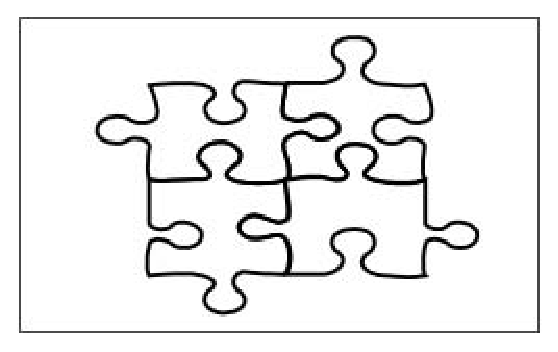
\includegraphics[height=4cm,width=6cm]{figs/fig1.eps}
  \end{center}
  \caption{ABC simulations to generate the Random Forest training database}
  \label{fig:abc-details}
\end{figure}

In a Bayesian context, when the likelihood function is too complex or untractable, several \emph{likelihood-free} methods are available to approximate it, including Approximate Bayesian Computation (ABC) \cite{marin2012approximate}. Given an observed data, the basic idea of ABC is to approximate the likelihood of a parametrized model with selected simulations, by comparing the observed data and simulated ones via computed \emph{summary statistics}. The table of summary statistics for simulated data is called \realemph{the reference table} (see fig. \ref{fig:abc-details}). It corresponds to the so called "training dataset" in Machine Learning terminology.

\subsection{ABC-RF posterior methodologies}
\label{sec:abc-post}

\subsubsection{Model Choice}
\label{sec:model-choice}

Given an observed data, and several (parametrized) models, the purpose is to estimate the best model to fit our data. A reference table combining summary statistics of simulated samples (particles) is generated from each model (models are sampled according a prior distribution, e.g. by penalizing the model complexity). A \emph{Model Choice} methodology is an inference method which takes this reference table, the observed data and \emph{infers} the best fitted model for this data, along with an estimated posterior probability (the probability of the model knowing the observed data), which assesses the fitness of the predicted model. 

\subsubsection{Parameter Estimation}
\label{sec:parameter-estimation}

Given an observed data and one parametrized model, the purpose is to infer one or several parameters for this model given the observed data. An ABC reference table is generated from the model. The \emph{Parameter estimation} methodology is an inference method which takes this reference table, the observed data and \emph{infers} one or several parameters, along with the usual Bayesian decorum : posterior distribution, quantiles and so on.

\subsubsection{General workflow}
\label{sec:worflow}

\begin{figure}
  \begin{center}
    \setlength{\unitlength}{5mm}
    % if you have pdflatex installed, you can use pdf files as graphics
    \includesvg[width=16cm]{figs/methodologies}
    % On the other hand, you must use eps files
    % 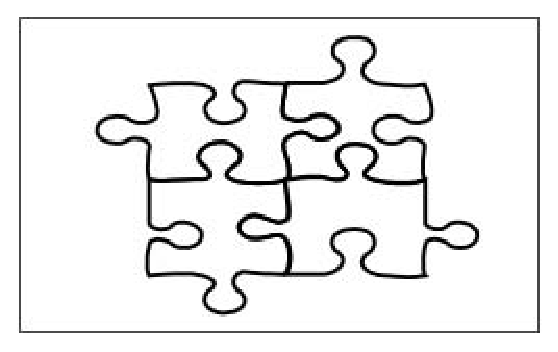
\includegraphics[height=4cm,width=6cm]{figs/fig1.eps}
  \end{center}
  \caption{Workflow with AbcRanger}
  \label{fig:abc-post}
\end{figure}

A sensible workflow is to first choose a model and then infer its parameters (see fig. \ref{fig:abc-post}).

\section{Second build block : Random Forests}
\label{sec:rf}

Enter the \emph{Supervised Machine Learning} (SML) realm \cite{friedman2001elements}: at the beginning lies a list a pair of input data/output data $\{x_i,y_i\}$ from $X$ and $Y$ domains, called a \emph{training dataset}. The objective is to \emph{learn} the best function $f_\theta{}(x)$ parametrized by 
$\theta\in\Theta$ so that a \emph{scalar loss function} $L : Y \times{} Y \mapsto \mathbb{R}$ is minimized on the $\Theta$ domain :

$$f_\theta{} = \underset{\theta{}}{\operatorname{argmin}}\ L(f(x_i),y_i)$$

Random Forests are based on CART, \emph{Classification and Regression Trees}, an algorithm developed by \cite{breiman:etal:1984}.

\subsection{CART}
\label{sec:cart}

% \begin{wrapfigure}{l}{0.5\textwidth}
  \begin{figure}
    \begin{center}
    \begin{tikzpicture}[scale=0.3, every node/.style={scale=1, minimum height=0.8cm}, thick]
      \useasboundingbox (-2,-2) rectangle (11.5,11);
      %\draw[very thin, gray] (0,0) grid[step=1] (10,10);

      \coordinate (c1) at (0,0);
      \coordinate (c2) at (0,10);
      \coordinate (c3) at (10,10);
      \coordinate (c4) at (10,0);

      \coordinate (X1) at (5,0);
      \coordinate (X2) at (0,5);

      \coordinate (cut1) at ($ (c1) + (0,4) $);
      \coordinate (cut1_bis) at ($ (c4) + (0,4) $);

      \coordinate (cut2) at ($ (c1) + (6,0) $);
      \coordinate (cut2_bis) at ($ (cut1) + (6,0) $);

      \coordinate (cut3) at ($ (cut1) + (3,0) $);
      \coordinate (cut3_bis) at ($ (c2) + (3,0) $);

      \coordinate (cut4) at ($ (cut3) + (0,4) $);
      \coordinate (cut4_bis) at ($ (cut1_bis) + (0,4) $);

      \coordinate (ret1) at (3,2);
      \coordinate (ret2) at (8,2);
      \coordinate (ret3) at (1.5,7);
      \coordinate (ret4) at (6.5,6);
      \coordinate (ret5) at (6.5,9);

      \coordinate (s1) at (0,4);
      \coordinate (s2) at (6,0);
      \coordinate (s3) at (3,0);
      \coordinate (s4) at (0,8);

      \draw (c1) -- (c2) -- (c3) -- (c4) -- (c1);
      \draw [color=lightblue,line width=1mm] (cut1) -- (cut1_bis);
      \draw [color=darkyellow,line width=1mm] (cut2) -- (cut2_bis);
      \draw [color=green!80!black,line width=1mm]  (cut3) -- (cut3_bis);
      \draw [color=red,line width=1mm] (cut4) -- (cut4_bis);

      \draw (ret1) node {$\hat{y}_1$};
      \draw (ret2) node {$\hat{y}_2$};
      \draw (ret3) node {$\hat{y}_3$};
      \draw (ret4) node {$\hat{y}_4$};
      \draw (ret5) node {$\hat{y}_5$};

      \draw [color=lightblue] (s1) node[left] {$s_1$};
      \draw [color=darkyellow] (s2) node[below] {$s_2$};
      \draw [color=green!80!black] (s3) node[below] {$s_3$};
      \draw [color=red] (s4) node[left] {$s_4$};

      \draw (s1) -- ++(-0.15,0);
      \draw (s2) -- ++(0,-0.15);
      \draw (s3) -- ++(0,-0.15);
      \draw (s4) -- ++(-0.15,0);

      \draw (X1) node[below, minimum height = 1.8cm] {$X_1$};
      \draw (X2) node[left, minimum width = 1.8cm] {$X_2$};

    \end{tikzpicture}%
    \begin{tikzpicture}[scale=0.5,
        edge from parent/.style={draw, thick, edge from parent path=
              {(\tikzparentnode.south)--+(0,-1.5pt)-| (\tikzchildnode)}},
        noeud/.style ={minimum size=1.2em, inner sep=4pt},
        level 1/.style={sibling distance=3cm},
        level 2/.style={sibling distance=2cm}]
      \tikzset{level distance=65pt}
      \node [noeud,color=lightblue] {$X_2 \leq s_1$}
      child {node [noeud,color=darkyellow] {$X_1 \leq s_2$}
          child {node [noeud] {$\hat{y}_1$} }
          child {node [noeud] {$\hat{y}_2$} }
        }
      child {node [noeud,color=green!80!black] {$X_1 \leq s_3$}
          child {node [noeud] {$\hat{y}_3$} }
          child {node [noeud,color=red] {$X_2 \leq s_4$}
              child {node [noeud] {$\hat{y}_4$} }
              child {node [noeud] {$\hat{y}_5$} }
            }
        };
    \end{tikzpicture}
  \end{center}
  \caption{An example of CART and the associated partition of the two dimensional predictor space. Each splitting condition takes the form $X_j \leq s$ and the prediction at a leaf is denoted $\hat{y}_\ell$.}
  \label{fig:CART-tree}
\end{figure}

A CART is a \emph{supervised machine learning algorithm} which essentially performs, recursively, a partitioning of the predictor space into disjoint subspaces. A prediction value is assigned to each of those subspaces (or \emph{Leaves}). Once the partitioning is done, the result is a binary tree which could predict outcomes from an input data, either classes or continuous values, by \emph{routing} the data to a \emph{leaf}, whose assigned value will be used then as prediction (see fig. \ref{fig:CART-tree}).

\subsection{Random Forests}
\label{sec:rf-explained}

\begin{figure}
  \begin{center}
    \setlength{\unitlength}{5mm}
    % if you have pdflatex installed, you can use pdf files as graphics
    \includesvg[width=14cm]{figs/RF}
    % On the other hand, you must use eps files
    % 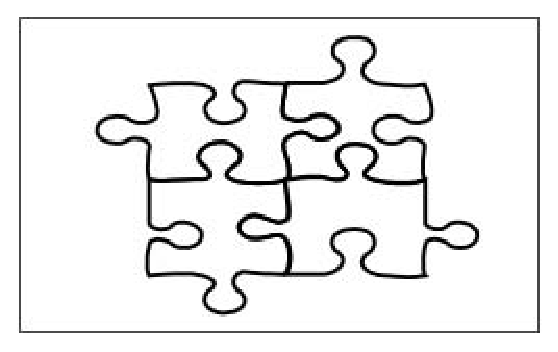
\includegraphics[height=4cm,width=6cm]{figs/fig1.eps}
  \end{center}
  \caption{Random Forest}
  \label{fig:rf-details}
\end{figure}

Random Forests \cite{breiman:2001} are a three pronged extension of CART (see fig. \ref{fig:rf-details}). First it is an \textbf{Ensemble method} which trains a \emph{set} of CART (not just one) and predict  the outcome with the  majority vote (resp. mean) of this set of trained trees for classification (resp. regression) target. Second, \textbf{bootstrapping} is applied before each tree training, i.e. training data is random sampled (with replacement). And last but not least, in a growing tree, at each node, the best split is computed on a \textbf{random subset of the features}. Those three extensions have multiple benefits; the main ones are lower variance compared to a single CART tree, due to the ensemble method, and \emph{unbiasedness}, because of the de-correlation of the trees induced by both bootstrapping and features random sampling. Other advantages are : robustness to noise, variable importance for (almost) free, integrated cross-validation procedure (out-of-bag samples, no need to get a validation dataset), easy parallelization, very good scaling properties (both in rows and columns axes), and provides both classification and regression target. 

\subsection{ABC Random Forest}
\label{sec:abcrf}

A reference implementation of the \emph{ABC-Random Forest} setup is given by \emph{abcrf} \cite{marinraynal2019abcrf}. We provide here a brief description of ABC Random Forest methodologies for model choice and parameter estimation.

\subsubsection{Model Choice}
\label{sec:abcrf-modelchoice}

Model Choice methodology in ABC-RF is two staged. \emph{First a classification random forest is trained} with the models (classes) as target. The trained random forest model is evaluated on the observed data, getting votes and the best model to fit. \emph{Second}, using the obtained random forest from the first stage, each sample from the training dataset is labeled classified/misclassified with the \emph{out-of-bag prediction} and finally as numerical 0 or 1 for a new target. Then, a \emph{new regression random forest} is trained on the training dataset, but this time with this new target (as continuous, non-categorical one for regression). And finally a prediction on the observed data is evaluated with the obtained random forest, and this predicted value (between 0 and 1) is a viable estimator for the \emph{posterior probability of the chosen model}.

\subsubsection{Parameter Estimation}
\label{sec:abcrf-estimparam}

In ABC Random Forest setup, parameter estimation is limited to one parameter at a time. Choosing a parameter $\theta$ to estimate, a regression RF is trained on a reference table generated only with the corresponding model and with the $\theta$ parameter values as target, forming the training dataset. Once trained, the regression RF is evaluated on the observed data and several outcomes are obtained, like an estimation of $\theta$, variance, and quantiles with the help of \textbf{quantile regression forests} \cite{meinshausen2006quantile}. It is worth noting that Quantile Forests are not new forests per se but an -- integrated -- method to compute weights distribution of the samples, knowing an observed (or out-of-bag) data. This distribution is then used to compute quantiles, for example. Finally a set of both prior et posterior estimators is inferred from the RF predictions, for example a prior (resp. posterior) \emph{pdf}, obtainable via standard kernel density estimation (resp. standard weighted density estimation).

\subsection{Linear augmentations}
\label{sec:linear}

As stated in \cite{pudlo2015reliable} (resp. \cite{raynal2016abc}), for Model choice (resp. parameter estimation), there is the option -- enabled by default --  to add linear combinations covariables to the existing summary statistics in the reference table via \emph{Linear Discriminant Analysis} (resp. \emph{Partial Least Squares}) \cite{friedman2001elements}. By refining the "square" partitioning of the trees, this sensibly improves the prediction accuracy of Random Forests outcomes, . 

\subsection{Computational limitations with ABC Random Forests reference implementation}
\label{sec:challenges-abcrf}

Faced with training dataset including ~100 000 lines and more than 10 000 summary statistics, \emph{abcrf} has been found growing trees over one gigabyte of memory size each. So, as typical random forests are made of 500 or 1000 trees for prediction performance, even with state of the art RF packages like \cite{wright2015ranger}, memory constraints are preventing completion of the training. 

This issue has a longer reach than an simple implementation issue and exhibits a fundamental mismatch of objectives between "classical" supervised machine learning setup and ABC posterior methodologies. Indeed, within "pure" SML, a model (like a Random Forest) is first trained, and then used to make predictions on a potentially endless source of new data; the whole model is stored by training and loaded in memory each time for prediction purpose. However, within the ABC inference context, the SML model is only needed for specific predictions directly on one or several observed data sample(s) and out-of-bag samples. Moreover, the corresponding trained Random Forest is coupled to the generated reference table (aka the training dataset), and is by no mean meant to generalize to new data (other reference tables), let alone other model and relevant observed data: in fact storing the forest is useless. Those remarks established the need of an adaptation of random forest algorithm for ABC.

\section{New implementation of Random Forest and ABC Random Forest}
\label{sec:new}

\begin{figure}
  \begin{center}
    \setlength{\unitlength}{5mm}
    % if you have pdflatex installed, you can use pdf files as graphics
    \includesvg[width=16cm]{figs/RF-optim}
    % On the other hand, you must use eps files
    % 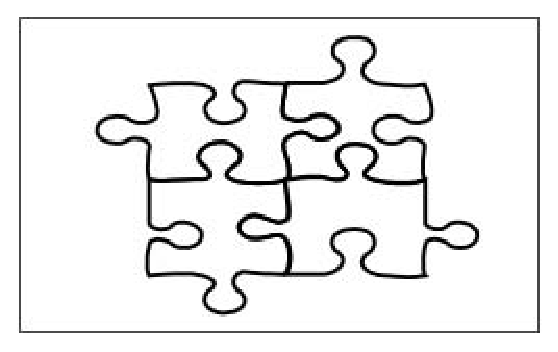
\includegraphics[height=4cm,width=6cm]{figs/fig1.eps}
  \end{center}
  \caption{Window of growing trees}
  \label{fig:rf-optim}
\end{figure}

Based on our own version of the core RF (written in C++) from the ranger package \cite{wright2015ranger}, our new implementation of Random Forest for ABC, \emph{AbcRanger}, solves the memory constraint issue related to the deep trees. Leveraging the cumulative nature of the ensemble method, Random Forest computations are now done in a \emph{joint grow/predict phase} for each tree, and then optimized in order to grow a limited batch of trees in memory. As illustrated by fig. \ref{fig:rf-optim}), this means that grow/predict computations for each tree is executed in a sequential –- i.e. batch-wise --  order: as now tree growing and predictions are computed in a single pass, predictions and posteriors are then stored/accumulated and each tree is finally discarded, freeing the system memory for next growing trees. The trees of the currently processed batch are still computed in parallel to leverage nowadays ubiquitous multicore architectures. 

Although this doesn't precludes the in-memory storage of the entire training dataset at once, this way of processing avoids the in-memory storage of the whole forest at no performance cost. In a very constrained memory environment, one should just have to lower the number of computing threads to keep the memory of a training batch in check. A special care has also been given to the Meinshausen's quantiles computations, completely parallelized and typically unnoticeable on multicore systems. Another advantage over \emph{abcrf} package: methodologies are now pure C++. So, it is relatively easy to provide wrappers/interfaces to other languages than R, like Python, with the added guarantee that no copy of the reference table happens between the core C++ layer handling the methodologies, and the interfaced language providing the reference table.

\subsection{A toy example application with the ELFI python package}

The \emph{ELFI} python package \cite{lintusaari2018elfi} provides a popular and flexible ABC framework, meant to integrate complex ABC and inferences pipelines. Inspired by the $Ma(2)$ toy example used by original ABC authors in \cite{marin2012approximate}, we used a more general $Ma(q)$ example for \href{https://github.com/diyabc/abcranger/blob/master/testpy/Model%20Choice%20Demo.ipynb}{model choice} and \href{https://github.com/diyabc/abcranger/blob/master/testpy/Parameter%20Estimation%20Demo.ipynb}{parameter estimation}, fixing $q=10$ in the following.

$MA(q)$ is a time series model defined by :

$$ x_{t}=\mu+\epsilon_{t}-\sum_{i=1}^{q} \vartheta_{i} \epsilon_{t-i} $$

For identifiability purposes the parameters should verify the following condition, roots of 

$$ Q(u)=1-\sum_{i=1}^{q} \vartheta_{i} u^{i} $$

should be strictly outside the (complex) unity disc, and this is our main prior constraint. Prior for $\theta_q$ is also sampled from an uniform distribution.

\begin{figure}
  \begin{center}
    \setlength{\unitlength}{5mm}
    % if you have pdflatex installed, you can use pdf files as graphics
    \includesvg[width=18cm]{figs/modelchoice-Signal}
    % On the other hand, you must use eps files
    % 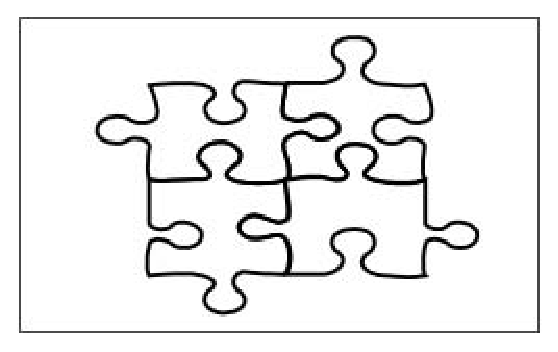
\includegraphics[height=4cm,width=6cm]{figs/fig1.eps}
  \end{center}
  \caption{Example of an $MA(10)$ model}
  \label{fig:signal}
\end{figure}

From the generated examples of $Ma(10)$ on a 200-length signal, sampling the prior $\theta_{10}$ uniformly in the $[1,2]$ interval, the usual row of (partial) autocorrelation features seems to be nonconclusive (see fig. \ref{fig:signal}) to discriminate between, for example $Ma(8)$, $Ma(10)$ or $Ma(12)$.

\subsubsection{Model choice: $Ma(10)$ vs "all" ($6 \leq q \leq 16$)}
\label{sec:modelchoice-all}

\begin{figure}
  \begin{center}
    \setlength{\unitlength}{5mm}
    % if you have pdflatex installed, you can use pdf files as graphics
    \includesvg[width=8cm]{figs/modelchoice-loop}
    % On the other hand, you must use eps files
    % 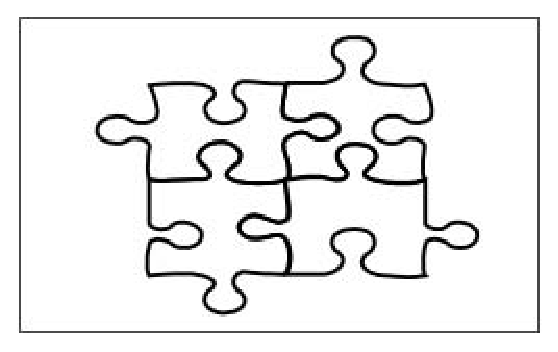
\includegraphics[height=4cm,width=6cm]{figs/fig1.eps}
  \end{center}
  \caption{Model Choice weighted histogram of inferred models: 100 $Ma(10)$ models are tried with ABC simulations followed by RF Model Choice inference (Signal length : 200 points, reftables : 2000 particles each).}
  \label{fig:modelchoice-loop}
\end{figure}

An ABC pipeline has been configured with \emph{elfi}, choosing the default sampler, without rejection  (option \verb+quantile+ fixed to $1$). For 100 trials, priors for $Ma(10)$ are sampled and observation generated, and models to choose are from $Ma(q)$ with $6 \leq q \leq 16$. On fig. \ref{fig:modelchoice-loop}, the performance of the ABC-RF setup is illustrated. 

\begin{figure}
  \begin{center}
    \setlength{\unitlength}{5mm}
    % if you have pdflatex installed, you can use pdf files as graphics
    \includesvg[width=8cm]{figs/modelchoice-rank}
    % On the other hand, you must use eps files
    % 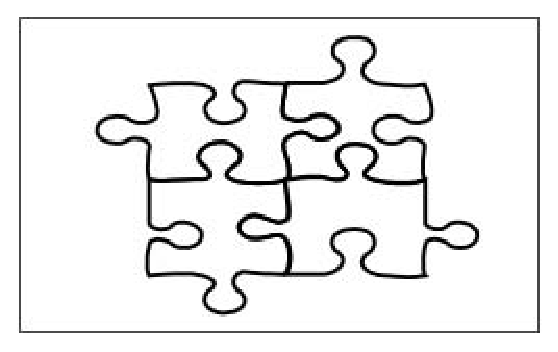
\includegraphics[height=4cm,width=6cm]{figs/fig1.eps}
  \end{center}
  \caption{10 most ranked summary statistics, sorted by permutation importance. \emph{$acf_i$, (resp. $pacf_i$, $pacf1_i$, $pacf2_i$)} are i-lagged autocorrelations (resp. partial autocorrelations, 0.05 and 0.95 corresponding quantiles).}
  \label{fig:rank}
\end{figure}

Also, features coming from $LDA$ linear augmentation  are discriminative, see fig. \ref{fig:rank} for one particular inference.

\subsubsection{Parameter Estimation}
\label{sec:paramestim-demo}

\begin{figure}
  \begin{center}
    \setlength{\unitlength}{5mm}
    % if you have pdflatex installed, you can use pdf files as graphics
    \includesvg[width=14cm]{figs/posterior-distrib}
    % On the other hand, you must use eps files
    % 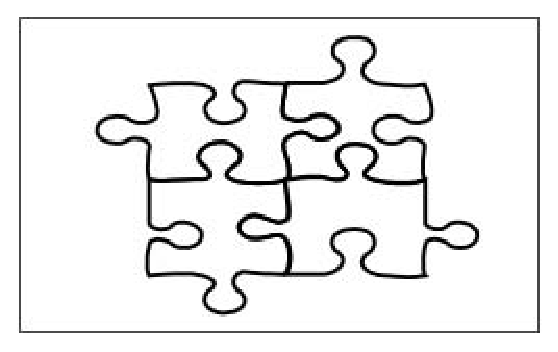
\includegraphics[height=4cm,width=6cm]{figs/fig1.eps}
  \end{center}
  \caption{Inferred posterior distributions of a $MA(10)$ model}
  \label{fig:posterior-distributions}
\end{figure}

For parameter estimation one $Ma(10)$ is sampled and observed, and then all parameters are inferred individually with ABC-RF methodology (whith the help of \emph{AbcRanger} python wrapper). Results are illustrated in fig. \ref{fig:posterior-distributions}. All parameters of the model were nicely estimated, and the posterior/prior distributions clearly discriminated.

\section{Conclusions and perspectives}
\label{sec:perspectives}

\emph{ABC-RF} posterior methodologies are a clean and efficient integration of SML techniques in a model-based approach, although the main objective is not the raw predictive power \emph{per se} like in a pure machine learning perspective, but easy to get, accurate and interpretable posteriors.

Many ideas emphasized in both posterior methodologies from \cite{pudlo2015reliable} and \cite{raynal2016abc} have strong connections with \emph{Generalized Random Forests} framework \cite{Athey_2019} we would like to explore in order to extend our developments to other fields than population genetics.

Moreover, we intend to pursue the algorithm adaptation of Random Forests for ABC even further, at the tree level: for a growing tree, only encountered leaves should be stored for point estimates and final moments. Thus, the memory footprint of the trees becomes negligible, and their growing could finally be parallelized at full scale.

Finally, by nature of Breiman's \emph{CART}, the computational bottleneck for random forests lies in the greedy, local split procedure at each node. To alleviate this, they are promising optimizations coming from the \emph{Gradient Boosted Trees} community \cite{ke2017lightgbm} and also some inspired by the \emph{Deep Learning} one like \cite{kontschieder2015deep}.

\bibliography{jobim_proceedings}

\end{document}
